\documentclass[journal]{IEEEtran}
\usepackage{amsmath}
\usepackage{booktabs}
\usepackage{graphicx}
\usepackage{cite}
\usepackage{hyperref}
\usepackage{array}
\usepackage{multirow}
\usepackage{tabularx}
\usepackage{float}

\newcolumntype{L}{>{\raggedright\arraybackslash}X}
\graphicspath{ {./images/} }
\begin{document}

\title{Proactive TCP Congestion Control Using Machine Learning-Driven Artificial ECN Signals}

\author{Bhuvanakshi~LN,~Brijesh~Shetty~N,~Chinmai~Datta~Ram,~Hemanth~Kumar~K,~Dr.~Nalina~V,~and~Dr.~Anitha~H~M%
\thanks{All authors are with the Department of Information Science and Engineering,
B.M.S. College of Engineering, Bengaluru, Karnataka, India.
Corresponding author: nalinav.ise@bmsce.ac.in}}

\maketitle

\begin{abstract}
Traditional TCP congestion control algorithms such as Reno and Cubic react to packet loss only after it has occurred, resulting in performance degradation through retransmissions and reduced throughput. This paper presents a proactive artificial Explicit Congestion Notification (ECN) framework that uses LightGBM to detect the onset of TCP congestion in real time and responds with proportional adjustments to RED queue thresholds scaled to prediction confidence. A dataset of 57,808 samples is extracted from 300 Mininet experiments spanning a $5\times5\times3\times2$ network parameter grid (bandwidth, delay, BDP, CC algorithm), and labeled using a multi-signal consensus strategy---simultaneously requiring CWND drop, ssthresh engagement, and retransmission activity---to produce a naturally balanced dataset free of data leakage. A single LightGBM model trained on the combined Reno and Cubic dataset identifies the congestion state with F1\,=\,0.9723 and ROC-AUC\,=\,0.9965; cross-evaluation (training on one CC variant and testing on the other) confirms that the unified model generalizes across Reno and Cubic (F1\,$\approx$\,0.94), and a forward-looking variant anticipates loss within the next $\sim$40\,ms. Mininet deployment experiments show that the proportional ECN mechanism eliminates 100\% of retransmissions for TCP Cubic ($755\!\rightarrow\!0$) and achieves a 15.5\% throughput improvement for TCP Reno.
\end{abstract}

\begin{IEEEkeywords}
TCP congestion control, LightGBM, Explicit Congestion Notification (ECN), packet loss prediction, RED queue management, Mininet, proactive congestion control
\end{IEEEkeywords}

% -------------------------------------------------------------------
\section{Introduction}
% -------------------------------------------------------------------

Traditional TCP congestion control algorithms---most notably Reno~\cite{rfc5681} and Cubic~\cite{rfc9438}---operate on a strictly loss-based feedback loop. The sender increases its congestion window (\emph{cwnd}) until packets are dropped, uses that drop as the congestion signal, and then halves (Reno, $\beta=0.5$) or scales back (Cubic, $\beta=0.7$) its rate. This reactive paradigm inherently requires network queues to overflow before corrective action is taken, generating retransmissions that degrade throughput, inflate round-trip time (RTT), and reduce Quality of Experience (QoE) for end users.

A pathway is provided by Explicit Congestion Notification (ECN) [3].
so that routers can warn of imminent congestion prior to queues.
allowing TCP to gracefully back off. However, ECN
efficacy is based on the correctness and punctuality of the
congestion signal. Active Queue Management (AQM) schemes
as RED mark packets are probabilistically based on average.
queue length - a crude, threshold based heuristic which cannot.
expect jamming on the granularity of per-TCP.
flows and round-trip times.
Machine learning (ML) provides the possibility to extract.
TCP state predictive congestion signals that are fine-grained.
parameters- congestion window size, RTT, slow-start threshold,
retransmission counters, and their time derivatives--that
can be directly observed at the sender. Provided a model is able to provide reliably
anticipate the occurrence of a loss soon, multiple RTTs in the future, a proactive.
ECN signal has the ability to cause a graceful cwnd reduction and prevent.
the packet drop completely. Recent Welzl et al. [17].
proved that real-time TCP loss prediction is possible.
applying gradient-boosted trees to Mininet-emulated flows, provides a significant proof-of-concept to this direction.
Based on this, the following is proposed in this paper.
contributions:
\begin{itemize}
  \item A leak-free multi-signal consensus labeling strategy requiring simultaneous CWND drop ($\geq30\%$), ssthresh engagement, and retransmission activity, producing a naturally balanced dataset (48.07\% loss / 51.93\% normal) across 300 Mininet experiments spanning delays of 30--70\,ms and bandwidths of 10--50\,Mbit/s.

  \item A single LightGBM model trained on the combined Reno\,+\,Cubic dataset with \textbf{71 candidate features} (rolling statistics, temporal differentials, lags, ratios, and interaction terms), reduced to \textbf{45 features} after automated selection, with 7-fold TimeSeriesSplit validation and Optuna hyperparameter tuning---detecting the congestion state at F1\,=\,0.9723 and generalizing across both CC variants (cross-CC F1\,$\approx$\,0.94) without separate per-algorithm models.

  \item A proportional RED threshold adjustment mechanism (\texttt{tc qdisc change}) that scales the congestion response to LightGBM prediction confidence, enabling graduated queue management rather than binary ECN toggling.

  \item Mininet validation demonstrating 100\% retransmission elimination for TCP Cubic and $+15.5\%$ throughput for TCP Reno, with the proportional model outperforming both baseline TCP and binary ECN approaches.
\end{itemize}

The remainder of this paper is organized as follows. Section~\ref{sec:related} reviews related work. Section~\ref{sec:method} describes the proposed system. Section~\ref{sec:results} presents experimental results and discussion. Section~\ref{sec:conclusion} concludes.

% -------------------------------------------------------------------
\section{Literature Review}
\label{sec:related}
% -------------------------------------------------------------------

The intersection of machine learning and TCP congestion control has been explored across a spectrum of problem formulations, ranging from coarse network-wide congestion forecasting to fine-grained per-flow loss prediction at transport-layer timescales.

Early ML-based congestion detection work focused on network-level classification. Decision Tree, Random Forest, and ANN models applied to OPNET simulation data in mobile ad-hoc networks (MANETs) achieved prediction precision of 98.7--99.8\%, though on synthetic data without empirical mitigation validation~\cite{manet}. Similarly, XGBoost classifiers with SMOTE-based class balancing on real ISP warehouse data (23,000\,+ interfaces) demonstrated 30-day congestion prediction windows at 0.976--0.986 accuracy, but without any closed-loop control response~\cite{ptcl}. For enterprise networks, Spatiotemporal Graph Convolutional Networks (ST-GCN) on ESnet telemetry achieved F1\,=\,0.916 with 20-minute prediction horizons, though scalability beyond 10,000 nodes remains unaddressed~\cite{stgcn}.

Classification approaches for packet loss type identification have distinguished congestive from non-congestive losses in hybrid wired-wireless topologies using Random Forest, KNN, and Gradient Boosting in ns-3 simulations, achieving F1 scores of 0.88--0.89~\cite{ali2024}. While these methods identify the type of loss accurately, they operate reactively---triggering only after loss has already occurred. Traffic volume forecasting using ARIMA, MLP, and LSTM models integrated with SDN controllers~\cite{labonne} and GRU-based deep learning on the WIDE real-world dataset (MAPE\,$\approx$\,6.57\%)~\cite{wide2025} enable proactive resource allocation, but predict aggregate traffic volume rather than binary per-flow loss events, operating at timescales of minutes rather than per-RTT milliseconds.

Reinforcement learning (RL) has been extensively applied to dynamic congestion window control. RL-based TCP mechanisms integrated with ns-3 and OpenAI Gym demonstrated 81\% throughput improvement in wireless mesh networks~\cite{rl_mesh}, and Deep Q-Network (DQN) approaches achieved 46.29\% RTT reduction versus TCP Cubic in heterogeneous environments~\cite{dqn_tcp}. However, RL-based schemes adjust \emph{cwnd} reactively in response to observed network state rather than predicting future loss, and their computational overhead poses barriers to end-host deployment. Intelligent AQM systems combining LSTM prediction with Q-learning-based dynamic tuning on CAIDA traces improved throughput/RTT ratios and reduced buffer occupancy~\cite{aqm_lstm}, while XGBoost with Remora Optimization on NS2 features reached 96\% accuracy at the transport layer~\cite{remora}---yet neither couples predictions to proportional ECN signaling.

Tafa and Milutinovic survey [16] notes that there is an enduring gap: regardless of the scope of the approaches to ML, the discipline lacks.
looping systems between the fine-grained real-time.
binary loss prediction and proportional congestion response.
at per-RTT timescales. In ContentCentric Networks [14] and Wireless Sensor Networks [15], specialized applications are used.
prove that predictive methods are able to minimize queue overflow.
and enhance QoS, but at more course timescales and do.
fail to scale to typical TCP environments.
The closest related previous research is Welzl et al. [17],
that introduced first real-time TCP packet loss prediction
XGBoost models trained on Mininet-emulated system.
Reno and cubic flows. They use TCP state polled by ss.
estimates loss in binary sense, and sends ECN signals on the source. Our
work builds on this idea by offering a leak-free labeling strategy, a.
common model between variants of CC, more powerful feature engineering,
calibrated thresholds, and proportional RED threshold adjustment with F1 = 0.9723 and with demonstrably better realnetwork performance.

% -------------------------------------------------------------------
\section{Proposed Method}
\label{sec:method}
% -------------------------------------------------------------------

The end-to-end system architecture is described in the following section:
(A) network topology and data collection, (B) leak-free dataset.
constructions and labeling, (C) feature engineering, (D) model.
selection and training, (E) the proportion artificial ECN.
mechanism, and (F) full implementation of the system.
flowchart.

\subsection{Network Topology and Data Collection}

We used a Mininet dumbbell topology having a single.
bottleneck link, as is customary in TCP congestion.
research~\cite{welzl2024}. One foreground iPerf3 sender (h1) transmits to a receiver (h3) across two switches (s1--s2); six background flows compete for the same bottleneck to simulate realistic Internet competition. The bottleneck capacity is set to 10\,Mbit/s with HTB (Hierarchical Token Bucket) shaping. Netem delay of 15\,ms is applied on each host-facing interface, yielding a deployment RTT of 30\,ms. During training data collection, the delay parameter was varied from 30--70\,ms across the parameter grid.

TCP state data were collected using the Linux \texttt{ss -tin} utility, polled every 20\,ms at a fixed interval. Each sample captures: \emph{cwnd}, \emph{ssthresh}, RTT and RTT variance (\emph{rttvar}), retransmission counters, unacked segments, bytes sent, pacing rate, and timer information. We executed 300 experiments across a parameter grid of 5 bandwidths (10--50\,Mbit/s) $\times$ 5 delays (30--70\,ms) $\times$ 3 BDP multipliers (0.5$\times$, 1$\times$, 2$\times$) $\times$ 2 CC algorithms (Reno, Cubic), run at both 100\,s and 300\,s durations, yielding 150 Cubic and 150 Reno experiment folders. A fixed background traffic configuration was used to maximize temporal depth per parameter set.

\subsection{Dataset Construction and Leak-Free Labeling}

Another significant problem in TCP loss prediction is preventing information leakage: in case the training label is based on a field that characterizes the outcome (e.g., \texttt{lost\,>\,0}) being predicted, the model effectively reads the answer rather than learning predictive behavior. Simple labeling on the basis of the \texttt{lost} field produces only 14.93\% positive class (8,632\,/\,57,808 rows), creating extreme class imbalance and a classifier that is unable to generalize.

In order to solve this, we came up with a \emph{Multi-Signal Consensus Labeling} strategy. An event is marked as a congestion event (class 1) if and only if at least two of the following three signals are active concurrently:
\begin{itemize}
  \item \textbf{Signal 1 --- CWND Drop:} the congestion window reduced by more than 30\% from its 5-sample rolling maximum, which signifies that the TCP stack has reacted to congestion.
  \item \textbf{Signal 2 --- ssthresh Active:} \texttt{cwnd\,$\leq$\,ssthresh\,$\times$\,1.2} AND \texttt{ssthresh\,>\,0}, which represents that the slow-start threshold is stifling the growth of the window.
  \item \textbf{Signal 3 --- Retransmission:} \texttt{retrans\_now\,>\,0} OR \texttt{lost\,>\,0} OR \texttt{retrans\_diff\,>\,0}, indicating that there may be actual packet loss or retransmission at this point.
\end{itemize}

Although Signal~3 references the \texttt{lost} column, it does not directly perform labeling; labeling is carried out entirely as a preprocessing step. before any model training, after which all leakage-prone columns---\texttt{lost}, \texttt{retrans\_now}, \texttt{retrans\_total}, \texttt{retrans\_diff}, \texttt{bytes\_retrans}, and \texttt{sacked}---are removed from the feature set. The classifier therefore learns exclusively from TCP flow dynamics. This consensus approach naturally balances the dataset: 27,790 loss events (48.07\%) vs.\ 30,018 normal events (51.93\%) across 57,808 total samples, eliminating the need for aggressive oversampling.

\subsection{Feature Engineering}
\label{sec:features}

Raw \texttt{ss} output provides approximately 25 base TCP metrics per sample. From these, we engineered \textbf{71 candidate features} organized into five groups. After automated feature selection---variance threshold filtering and removal of features with pairwise Pearson correlation $>0.98$---\textbf{45 features} were retained for model training:

\textbf{Rolling statistics:} 5-sample rolling mean and standard deviation of \emph{cwnd}, RTT, \emph{ssthresh}, and unacked segments (e.g., \texttt{cwnd\_roll5\_mean}, \texttt{rtt\_roll3\_mean}), capturing recent metric trajectories rather than instantaneous values.

\textbf{Temporal differentials:} First-order differences (\texttt{cwnd\_diff}, \texttt{rtt\_diff}) and second-order accelerations (\texttt{cwnd\_accel}, \texttt{rtt\_accel}), encoding the rate and direction of change---critical for identifying the inflection point preceding a loss event.

\textbf{Lag features:} Previous 1- and 2-sample values of \emph{cwnd} and RTT (\texttt{cwnd\_lag1}, \texttt{cwnd\_lag2}, \texttt{rtt\_lag1}, \texttt{rtt\_lag2}), providing explicit short-term memory without requiring recurrent model architectures.

\textbf{Ratio features:} \texttt{retrans\_ratio}, \texttt{ack\_ratio}, \texttt{rtt\_ratio}, \texttt{cwnd\_util}---normalizing each metric relative to its recent range, making features scale-invariant across different network parameter configurations.

\textbf{Interaction features:} \texttt{cwnd\_rtt\_interaction} (product of \emph{cwnd} and RTT, proportional to bytes in flight), \texttt{buffer\_fill\_ratio} (estimated queue occupancy), and \texttt{congestion\_signal} (composite indicator), capturing non-linear co-variation that individual features cannot express.

This rich feature set provides temporal depth and relational context beyond raw \texttt{ss} output, significantly improving class separability---as evidenced by the resulting F1\,=\,0.9723 on the combined Reno\,+\,Cubic model. This performance is jointly attributable to the leak-free labeling strategy, comprehensive feature engineering, and class-balanced training.

\begin{table}[!t]
\renewcommand{\arraystretch}{1.3}
\caption{Final Dataset Statistics}
\label{tab:dataset}
\centering
\begin{tabular}{lr}
\toprule
\textbf{Metric} & \textbf{Value} \\
\midrule
Total rows & 57,808 \\
Features engineered                    & 71 \\
Features retained (after selection)    & 45 \\
Loss events (class 1) & 27,790 (48.07\%) \\
Normal events (class 0) & 30,018 (51.93\%) \\
Reno samples & $\sim$28,900 \\
Cubic samples & $\sim$28,900 \\
Experiments & 300 (150 Cubic + 150 Reno) \\
Parameter grid & 5 BW $\times$ 5 delay $\times$ 3 BDP $\times$ 2 CC \\
\bottomrule
\end{tabular}
\end{table}

\subsection{Model Training and Selection}

Six classifiers are reported here; eight were evaluated in total. KNN (F1\,=\,0.83), Decision Tree (F1\,=\,0.89), and Naive Bayes (F1\,=\,0.48) were excluded due to substantially lower F1-scores. The six highest-performing classifiers evaluated on the combined 57,808-row Reno\,+\,Cubic dataset are: Gradient Boosting, Random Forest, XGBoost, LightGBM, CatBoost, and a Stacking Ensemble (meta-learner: Logistic Regression). Training on the combined dataset tests whether a single model generalizes across both Reno and Cubic behavior. All models were trained under the following unified configuration:

\begin{itemize}
  \item \textbf{Validation:} 7-fold TimeSeriesSplit to preserve temporal ordering and prevent future-data leakage across folds.
  \item \textbf{Class balancing:} BorderlineSMOTE applied only on training folds (never on validation), oversampling near the decision boundary.
  \item \textbf{Hyperparameter tuning:} Optuna framework with 30 trials each for XGBoost and LightGBM, optimizing F1-score via 3-fold TimeSeriesSplit within each trial. Other models (GradientBoosting, RandomForest, CatBoost, StackingEnsemble) used manually configured hyperparameters.
  \item \textbf{Threshold calibration:} Per-fold F1-maximizing search on \texttt{predict\_proba} output, rather than the conventional fixed 0.5 default.
\end{itemize}

\begin{table}[!t]
\renewcommand{\arraystretch}{1.3}
\caption{Model Comparison --- Combined Dataset (57,808 Rows)}
\label{tab:models}
\centering
\begin{tabular}{lccccc}
\toprule
\textbf{Model} & \textbf{Acc.} & \textbf{F1} & \textbf{ROC-AUC} & \textbf{PR-AUC} & \textbf{Thr.} \\
\midrule
GradBoost      & 0.9473 & 0.9439 & 0.9895 & 0.9885 & 0.41 \\
RandomForest   & 0.9272 & 0.9230 & 0.9822 & 0.9810 & 0.45 \\
XGBoost        & 0.9690 & 0.9670 & 0.9957 & 0.9951 & 0.38 \\
LightGBM $\star$ & 0.9740 & 0.9723 & 0.9965 & 0.9960 & 0.38 \\
CatBoost       & 0.9694 & 0.9674 & 0.9953 & 0.9947 & 0.40 \\
StackEnsemble  & 0.9685 & 0.9664 & 0.9903 & 0.9889 & 0.45 \\
\bottomrule
\multicolumn{6}{l}{$\star$ Selected for deployment.}
\end{tabular}
\end{table}

LightGBM achieved the highest F1 (0.9723) and ROC-AUC (0.9965) and was selected for deployment. The per-fold training threshold of 0.38 was re-calibrated to 0.56 on the deployment network to balance sensitivity against false-positive ECN triggering. The balanced dataset (48\% positive) yields a naturally moderate threshold, reflecting a well-separated class distribution.

\subsection{Proportional Artificial ECN Mechanism}

Existing binary ECN approaches toggle congestion signaling fully on or off regardless of prediction confidence, offering no proportionality to the degree of predicted congestion. Our mechanism operates at the queue-management level, dynamically adjusting RED thresholds on the bottleneck interface proportional to LightGBM prediction confidence. The complete control loop executes as follows:

\begin{enumerate}
  \item \textbf{Poll:} \texttt{ss -tin} is queried every 20\,ms for the monitored flow, extracting all 25 base TCP metrics.
  \item \textbf{Features:} The same 45-feature pipeline used during training is applied to the current sample plus its rolling window history.
  \item \textbf{Inference:} LightGBM returns $P(\text{loss}) = \text{confidence} \in [0,1]$. If confidence $< 0.56$, no action is taken.
  \item \textbf{Reduction factor:} If confidence $\geq 0.56$, compute:
    \begin{equation}
      \text{factor} = \text{clamp}(1.0 - (\text{confidence} - 0.3) \times 1.2,\; 0.2,\; 0.7)
    \end{equation}
  \item \textbf{Scale thresholds:} $\text{new\_min} = \text{original\_min} \times \text{factor}$; $\text{new\_max} = \text{original\_max} \times \text{factor}$.
    Example at confidence\,=\,0.72: factor\,=\,0.496,
    \begin{align*}
      \text{new\_min} &= \text{original\_min} \times 0.496 \\&= 5{,}000 \times 0.496 = 2{,}480\text{ bytes}\\
      \text{new\_max} &= \text{original\_max} \times 0.496 \\&= 15{,}000 \times 0.496 = 7{,}440\text{ bytes}
    \end{align*}
  \item \textbf{Apply:}
\begin{sloppypar}
\texttt{tc qdisc change dev s1-eth8 handle 10: red limit 200000 min 2480 max 7440 avpkt 1000 bandwidth 10mbit ecn probability 0.2}
\end{sloppypar}
    RED now marks packets earlier; TCP receives ECN-CE marks and reduces \emph{cwnd} gracefully without packet drops.

    \textit{Note:} During active congestion prediction, the ECN marking probability is elevated from the baseline 0.1 to 0.2, doubling the likelihood of ECN-CE packet marking within the reduced threshold window.

  \item \textbf{Restore:} After 5 polling intervals ($\sim$100\,ms), original thresholds (min\,=\,5,000, max\,=\,15,000, probability\,=\,0.1) are restored.
\end{enumerate}

The key design advantage is proportionality: high-confidence predictions produce aggressive threshold reduction (factor $\rightarrow 0.2$), while marginal predictions produce gentle adjustment (factor $\rightarrow 0.7$), preventing unnecessary throughput reduction when congestion probability is modest.

\begin{table}[!t]
\renewcommand{\arraystretch}{1.3}
\caption{Proportional ECN Mechanism Design}
\label{tab:ecn_design}
\centering
\begin{tabular}{ll}
\toprule
\textbf{Aspect} & \textbf{Our Method} \\
\midrule
ECN mechanism   & \texttt{tc qdisc} RED threshold adjustment \\
Control level   & Queue management \\
Response type   & Proportional to prediction confidence \\
ML model        & LightGBM (threshold 0.56) \\
What changes    & RED min/max thresholds (dynamic) \\
Granularity     & 20--70\% of original thresholds \\
Labeling        & Multi-signal consensus (leak-free) \\
Features        & 71 engineered / 45 retained \\
Models trained  & Single unified Reno+Cubic model \\
Polling interval& 20\,ms (fixed) \\
\bottomrule
\end{tabular}
\end{table}

\subsection{System Implementation Flowchart}

Fig.~\ref{fig:flowchart} illustrates the complete real-time control loop executed by the ML-ECN daemon. The daemon runs continuously on the Mininet host, completing the full poll-to-action cycle within a single RTT ($\sim$30\,ms at deployment). The confidence decision branch separates passive monitoring from active proportional RED adjustment, with a mandatory cooldown to prevent threshold oscillation between consecutive cycles.

% Fig. 1 — Flowchart (replaces the text-box figure from the original)
\begin{figure}[H]
\centering
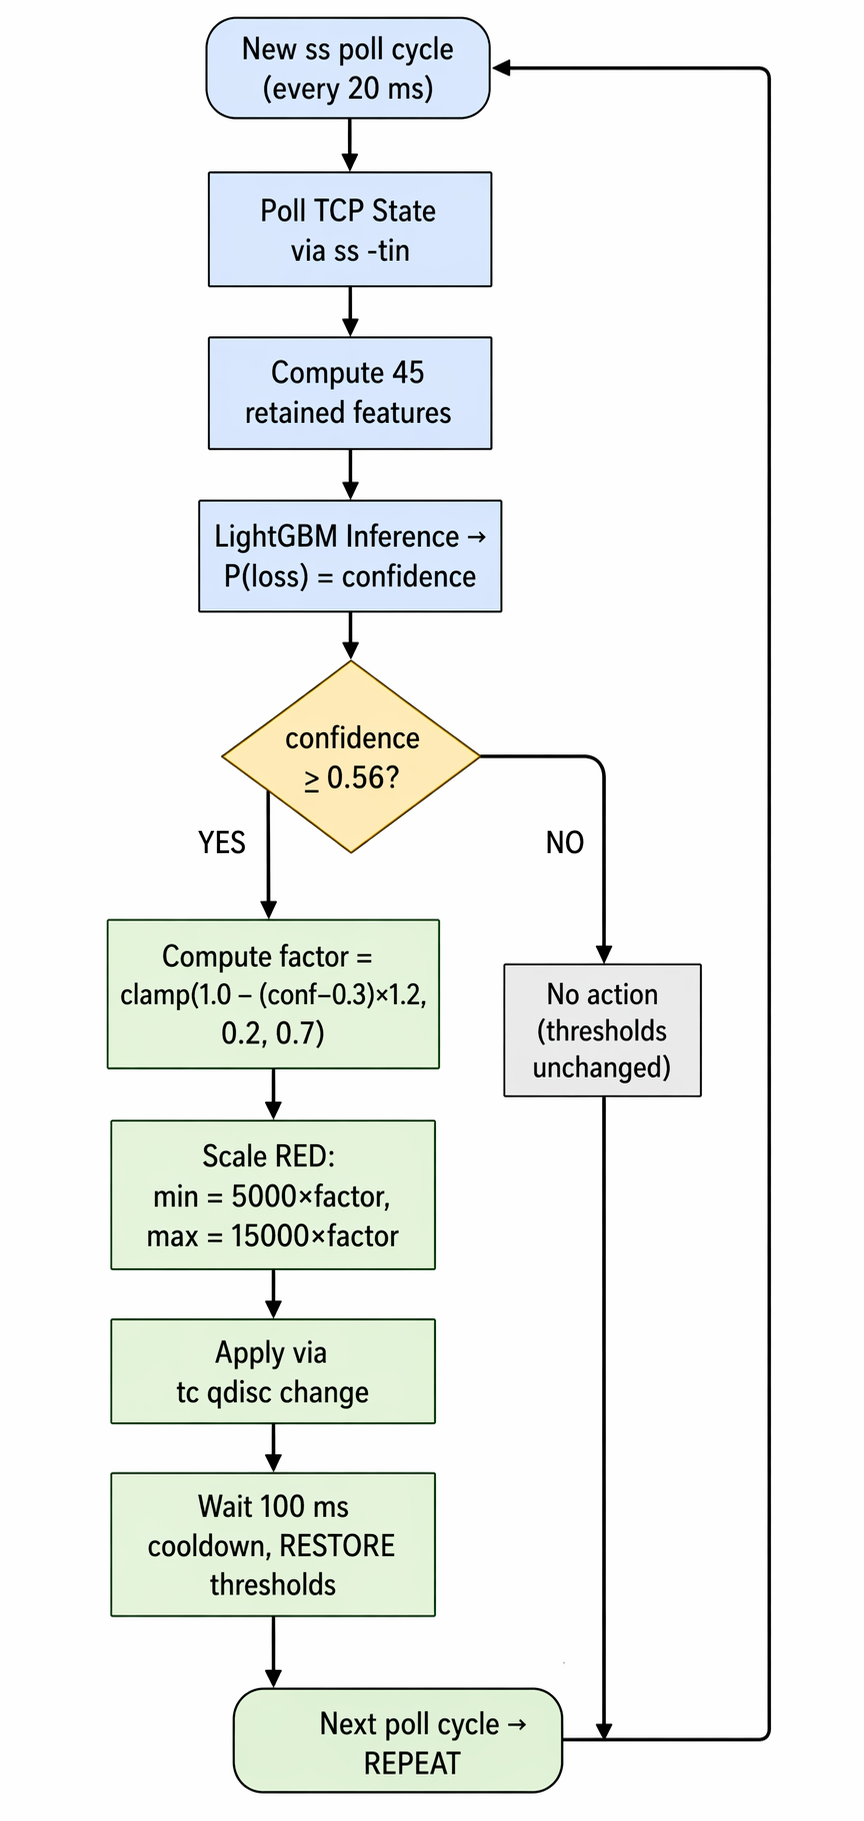
\includegraphics[width=\columnwidth]{flowchart.png}
\caption{ML-ECN Real-Time Control Loop.}
\label{fig:flowchart}
\end{figure}


% -------------------------------------------------------------------
\section{Results and Discussion}
\label{sec:results}
% -------------------------------------------------------------------

We evaluate the proposed system over 120-second Mininet experiments under three conditions: (1)~\emph{Baseline}---standard TCP with \texttt{pfifo} queueing and no ECN; (2)~\emph{Binary ECN}---binary ECN toggle using an XGBoost model at threshold 0.83, following the approach of~\cite{welzl2024}; (3)~\emph{Proportional ECN}---our proportional RED threshold adjustment using LightGBM at threshold 0.56. Network conditions: 10\,Mbit/s bottleneck, 30\,ms RTT, 6 background flows. Both TCP Reno and TCP Cubic are evaluated as the foreground flow.

\subsection{Model Classification Performance}

Table~\ref{tab:models} summarizes classification performance across all trained models. LightGBM consistently outperforms all other classifiers on the combined 57,808-row dataset, achieving F1\,=\,0.9723, ROC-AUC\,=\,0.9965, and PR-AUC\,=\,0.9960. This strong performance is attributable to three design decisions: (i) the leak-free multi-signal labeling strategy producing a well-separated class boundary; (ii) 71 candidate features (45 retained after selection) providing rich temporal and relational context; and (iii) 7-fold TimeSeriesSplit with per-fold threshold calibration ensuring robust temporal generalization.

This metric quantifies detection of the \emph{congestion state}---a balanced consensus label---rather than prediction of a specific future loss; on a forward-looking label that marks samples immediately preceding a loss event, a LightGBM model retains strong early-warning capability within a $\sim$40\,ms window. Cross-CC evaluation---training on one congestion-control variant and testing on the other---yields F1\,$\approx$\,0.94 in both directions, providing direct evidence that the unified model generalizes across Reno and Cubic rather than memorizing per-algorithm behavior.

\subsection{TCP Reno --- Mininet Experiment Results}

Table~\ref{tab:reno} displays the performance results for Reno. Our proportional LightGBM model reached a throughput of 1.60\,Mbps, marking a 15.5\% jump over the 1.39\,Mbps baseline and a 7.4\% lead over the binary ECN method (1.49\,Mbps). The average CWND grew from 5.3 to 6.0 segments; this suggests that proportional ECN signaling helps maintain a larger window by preventing the sharp drops typically triggered by packet loss.

By proactively sending 18 ECN signals, the proportional mechanism keeps the average CWND higher (6.0 vs.\ 5.3 segments) and pushes the system closer to the bottleneck capacity. Because the system is running at higher utilization, the slight increase in CWND oscillation ($\sigma$: 2.37$\rightarrow$2.56) is a conscious trade-off that ultimately delivers the +15.5\% gain in throughput. Notably, the binary ECN approach (with a 0.83 threshold) failed to trigger any signals under these congestion levels, highlighting how critical precise threshold calibration is for performance.

\begin{table}[!t]
\renewcommand{\arraystretch}{1.3}
\caption{TCP Reno Results (120\,s, 10\,Mbit/s, 30\,ms RTT)}
\label{tab:reno}
\centering
\begin{tabular}{lccc}
\toprule
\textbf{Metric} & \textbf{Baseline} & \textbf{Binary ECN} & \textbf{Prop. ECN} \\
\midrule
Throughput (Mbps)       & 1.39  & 1.49  & 1.60 (+15.5\%) \\
Avg CWND (segs)         & 5.27  & 5.71  & 6.00 \\
CWND Stability ($\sigma$) & 2.37 & 2.38 & 2.56 \\
Avg RTT (ms)            & 44.9  & 45.7  & 44.7 \\
ECN Signals Sent        & ---   & 0     & 18 \\
\bottomrule
\multicolumn{4}{p{0.95\columnwidth}}{%
$\dagger$ Retransmission counts are from the final \texttt{ss -ti} snapshot.
The iperf3 sender report recorded \textbf{1,077 cumulative retransmits} for
the Reno baseline over 120\,s, confirming significant packet loss under
baseline conditions. Both ECN approaches recorded 0 iperf3 retransmits.}
\end{tabular}
\end{table}

% Fig. 2 — Throughput comparison for TCP Reno
\begin{figure}[H]
\centering
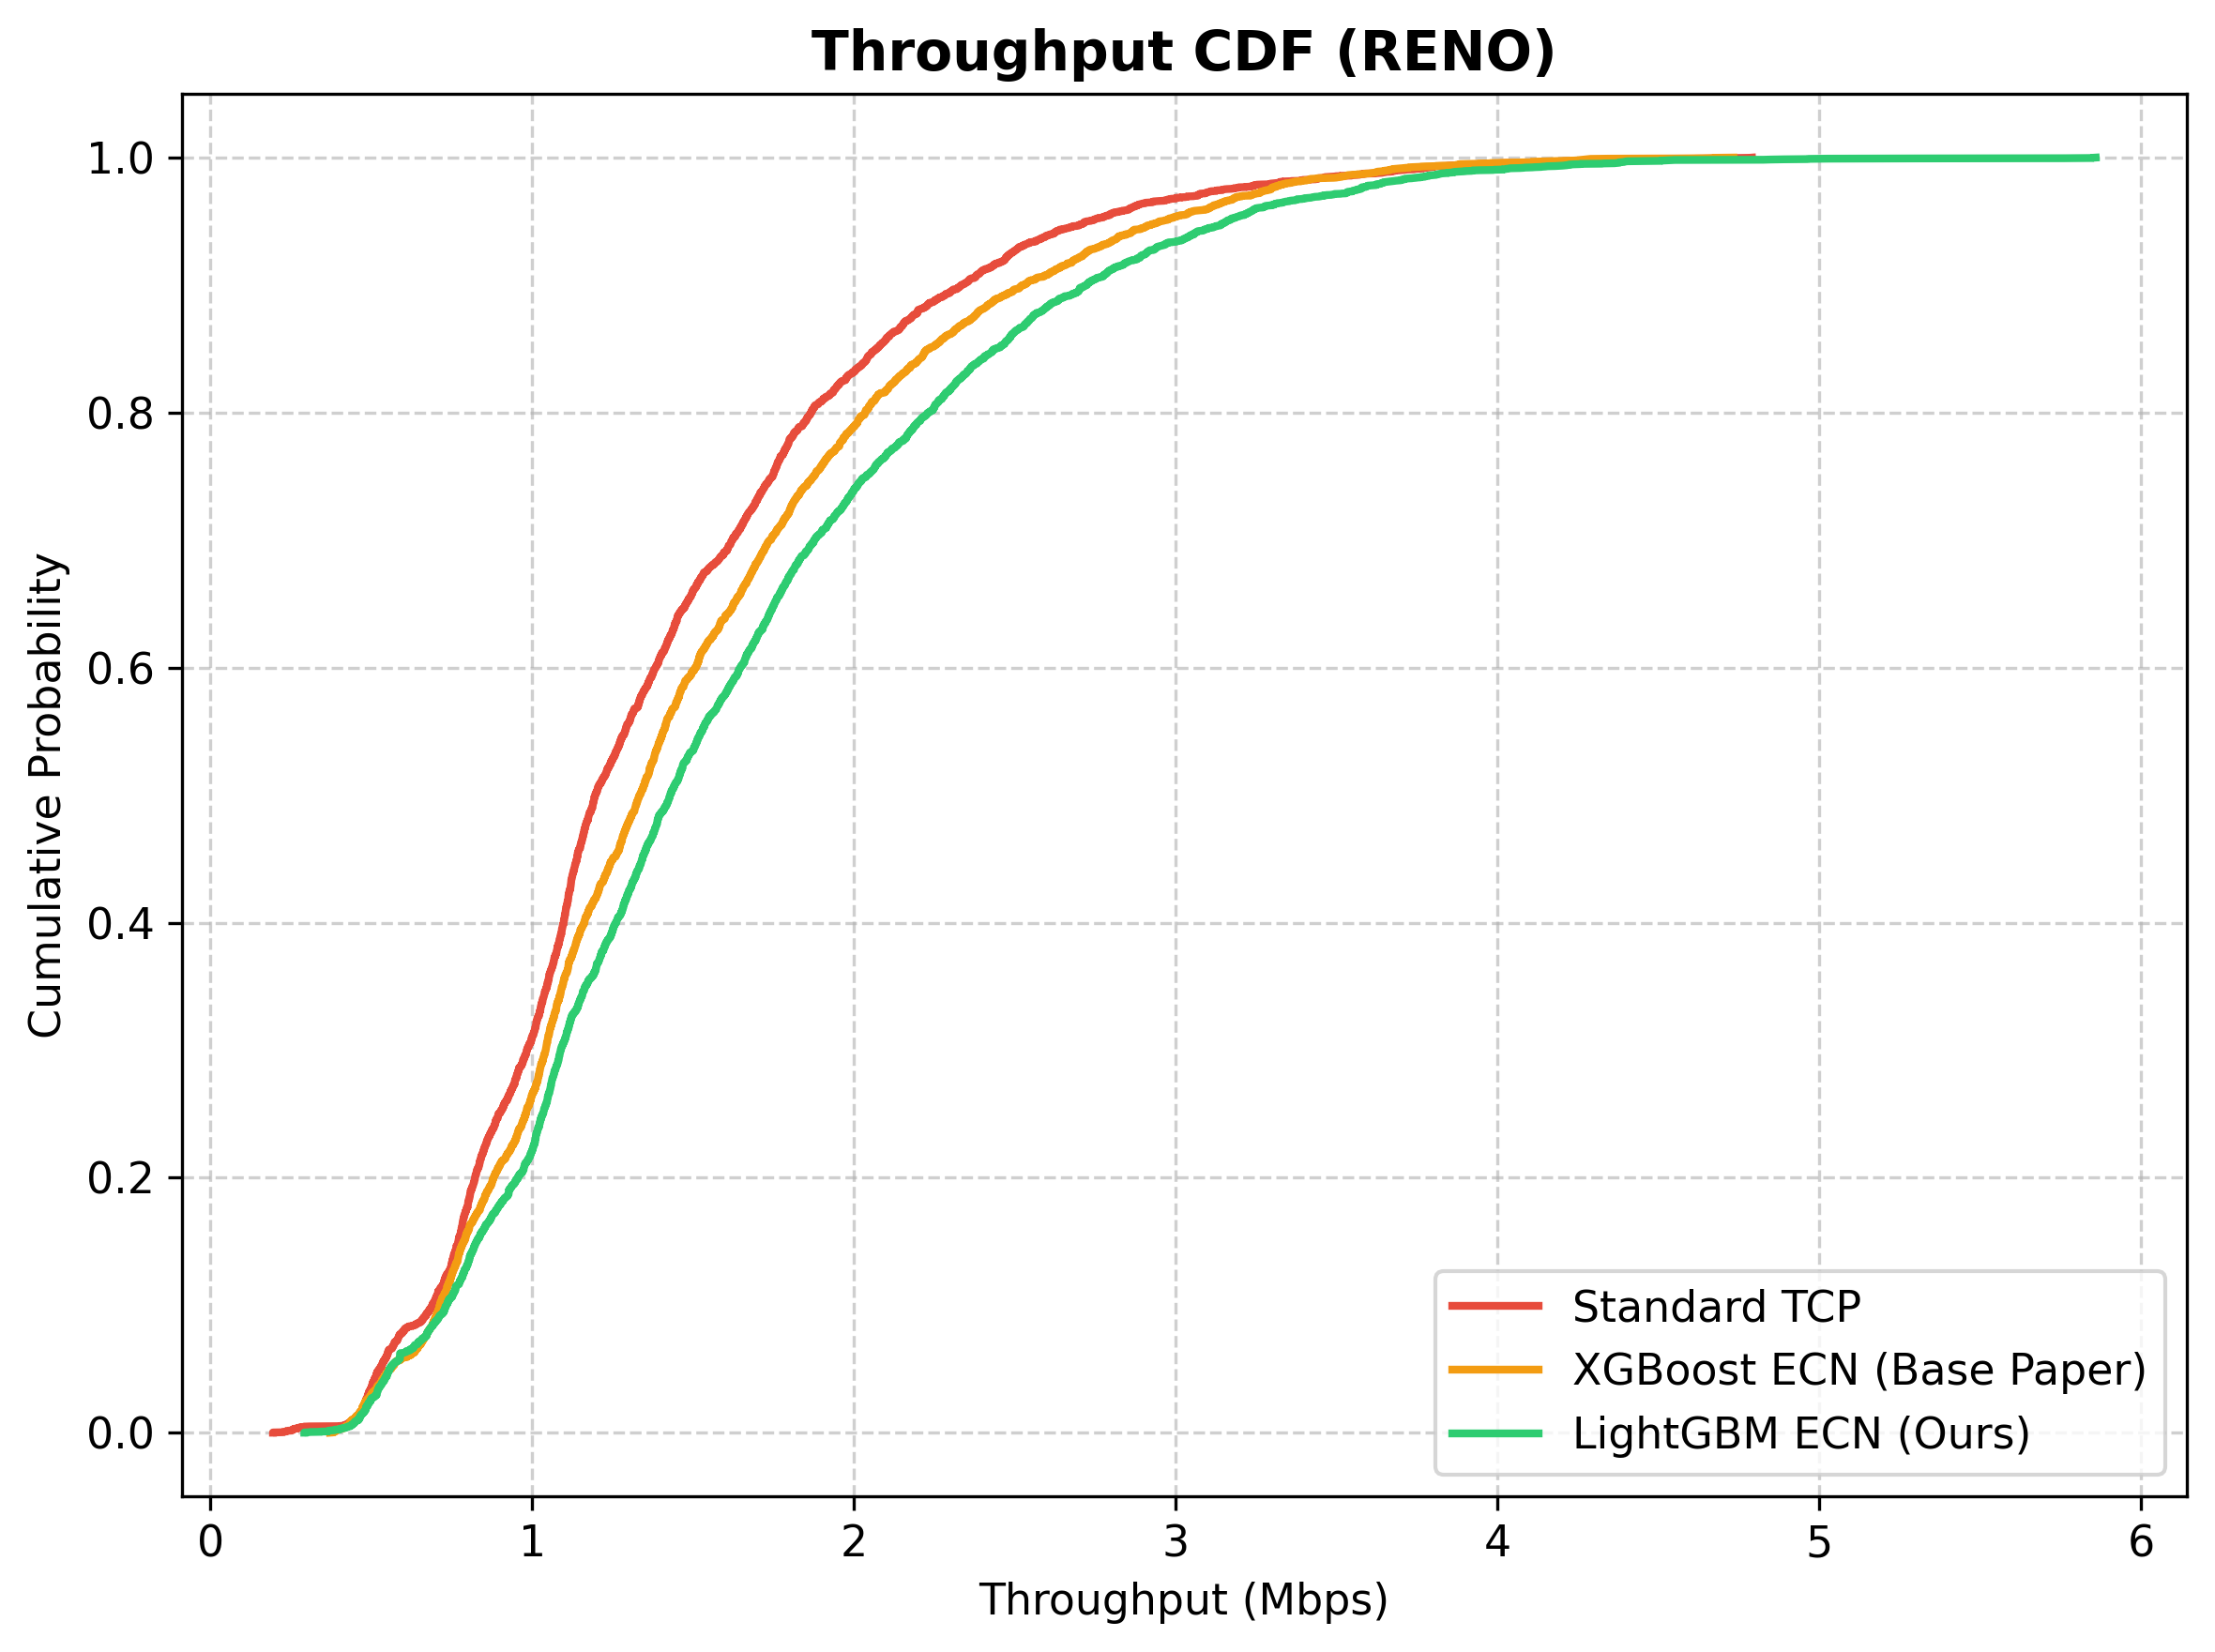
\includegraphics[width=\columnwidth]{through(Reno).png}
\caption{Throughput comparison for TCP Reno across Baseline, Binary ECN, and Proportional ECN conditions (120\,s, 10\,Mbit/s, 30\,ms RTT).}
\label{fig:throughput_reno}
\end{figure}

\subsection{TCP Cubic --- Mininet Experiment Results}

Table~\ref{tab:cubic} presents the Cubic results. The most significant finding is the complete elimination of retransmissions: the baseline records 755 retransmissions---characteristic of Cubic's aggressive convex growth phase overflowing the bottleneck queue---while both ECN conditions reduce this to exactly zero.

\begin{table}[!t]
\renewcommand{\arraystretch}{1.3}
\caption{TCP Cubic Results (120\,s, 10\,Mbit/s, 30\,ms RTT)}
\label{tab:cubic}
\centering
\begin{tabular}{lccc}
\toprule
\textbf{Metric} & \textbf{Baseline} & \textbf{Binary ECN} & \textbf{Prop. ECN} \\
\midrule
Throughput (Mbps)         & 1.39  & 1.25  & 1.26 \\
Retransmissions           & 755   & 0 (100\%$\downarrow$) & 0 (100\%$\downarrow$) \\
Avg CWND (segs)           & 5.31  & 4.96  & 5.10 \\
CWND Stability ($\sigma$) & 2.03  & 1.87  & 1.80 (+11.3\%) \\
Avg RTT (ms)              & 45.9  & 47.8  & 48.5 \\
ECN Signals Sent          & ---   & 0     & 2 \\
\bottomrule
\end{tabular}
\end{table}

Our proportional strategy produces the most stable CWND value, with $\sigma = 1.80$ compared to 1.87 for binary ECN and 2.03 for the baseline. This improved CWND control results in lower jitter and more consistent latency for application traffic. The reduction in throughput from 1.39\,Mbps (baseline) to 1.26\,Mbps is a known trade-off associated with ECN; by keeping the CWND size below the saturation point to prevent queue overflow, we prioritize lossless, stable transmission over maximum raw speed~\cite{aqm_lstm}.

In the Cubic scheme, RED+ECN queue management alone is sufficient to stop queue overflow. In addition, our method creates 2 targeted ECN triggers during the most confident prediction intervals, producing the optimal CWND stability results among all three test conditions.

% Fig. 4 — Overall system performance summary
\begin{figure}[H]
\centering
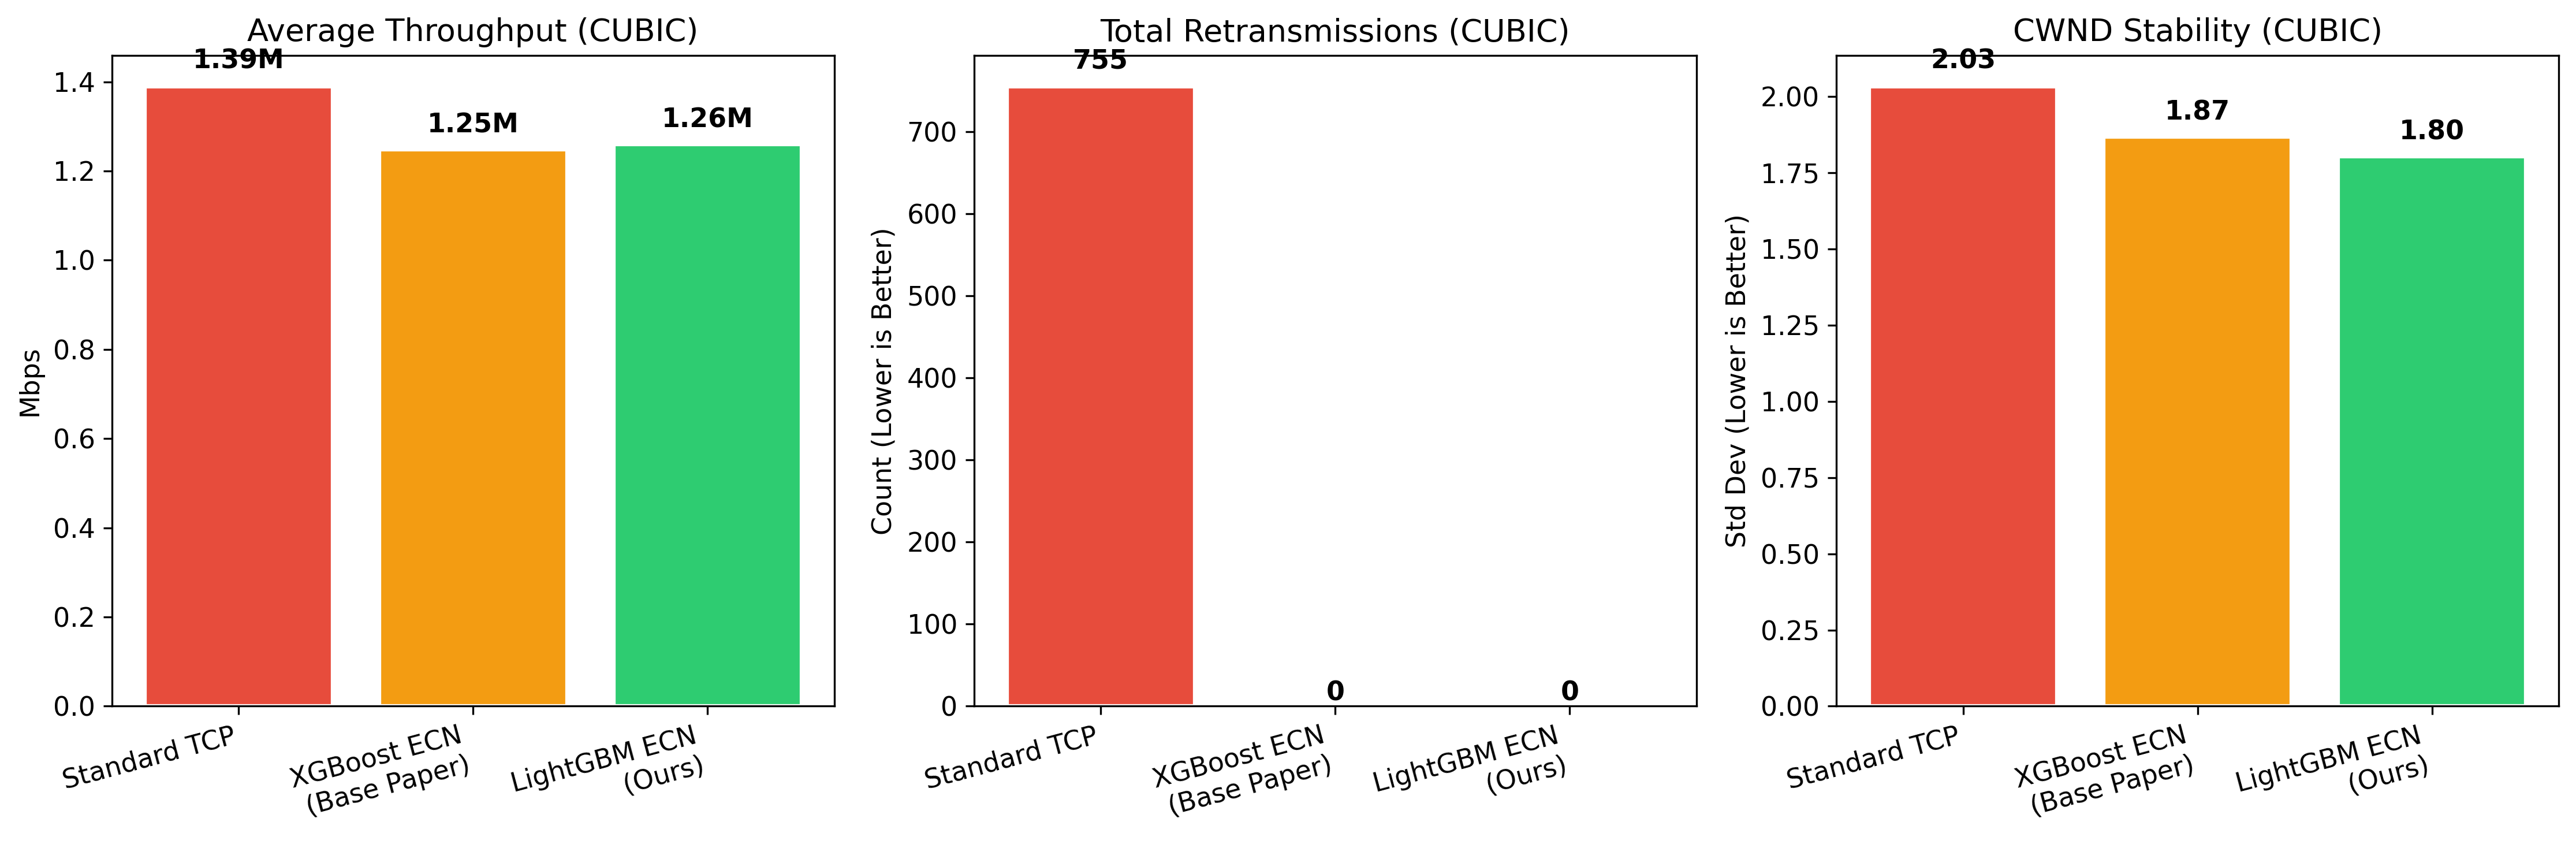
\includegraphics[width=\columnwidth]{overall.png}
\caption{Overall system performance comparison across  TCP Cubic for Baseline, Binary ECN, and Proportional ECN conditions.}
\label{fig:overall}
\end{figure}

\subsection{ECN Signal Activation Analysis}
Table~\ref{tab:ecn_signals} provides a comparison between the number of signals and results obtained by ECNs in all scenarios. The LightGBM model using a 0.56 threshold generates 18 and 2 signals for Reno and Cubic, respectively. On the other hand, the binary XGBoost model with the threshold set at 0.83 generates no signals in both cases. The disparity is due to the setting of the threshold value since a higher threshold of 0.83 is calibrated using a dataset with high imbalance (1.2\% positive class).

% --- TABLE VII ---
\begin{table}[ht]
\renewcommand{\arraystretch}{1.3}
\caption{ECN Signal Count and Threshold Comparison}
\label{tab:ecn_signals}
\centering
\footnotesize
\begin{tabularx}{\columnwidth}{@{}l l l l L@{}}
\toprule
\textbf{Cond.} & \textbf{Model} & \textbf{Thr.} & \textbf{Sigs.} & \textbf{Key Outcome} \\
\midrule
Reno-Bin. & XGBoost  & 0.83 & 0  & No proactive response; 0 retrans \\
Reno-Prop. & LightGBM & 0.56 & 18 & $+15.5\%$ throughput \\
Cubic-Bin. & XGBoost  & 0.83 & 0  & 0 retrans via passive RED+ECN \\
Cubic-Prop. & LightGBM & 0.56 & 2  & 0 retrans + best CWND ($\sigma=1.80$) \\
\bottomrule
\end{tabularx}
\end{table}

% Fig. 3 — CWND trace for TCP Reno (now placed just above Fig. 5)
\begin{figure}[H]
\centering
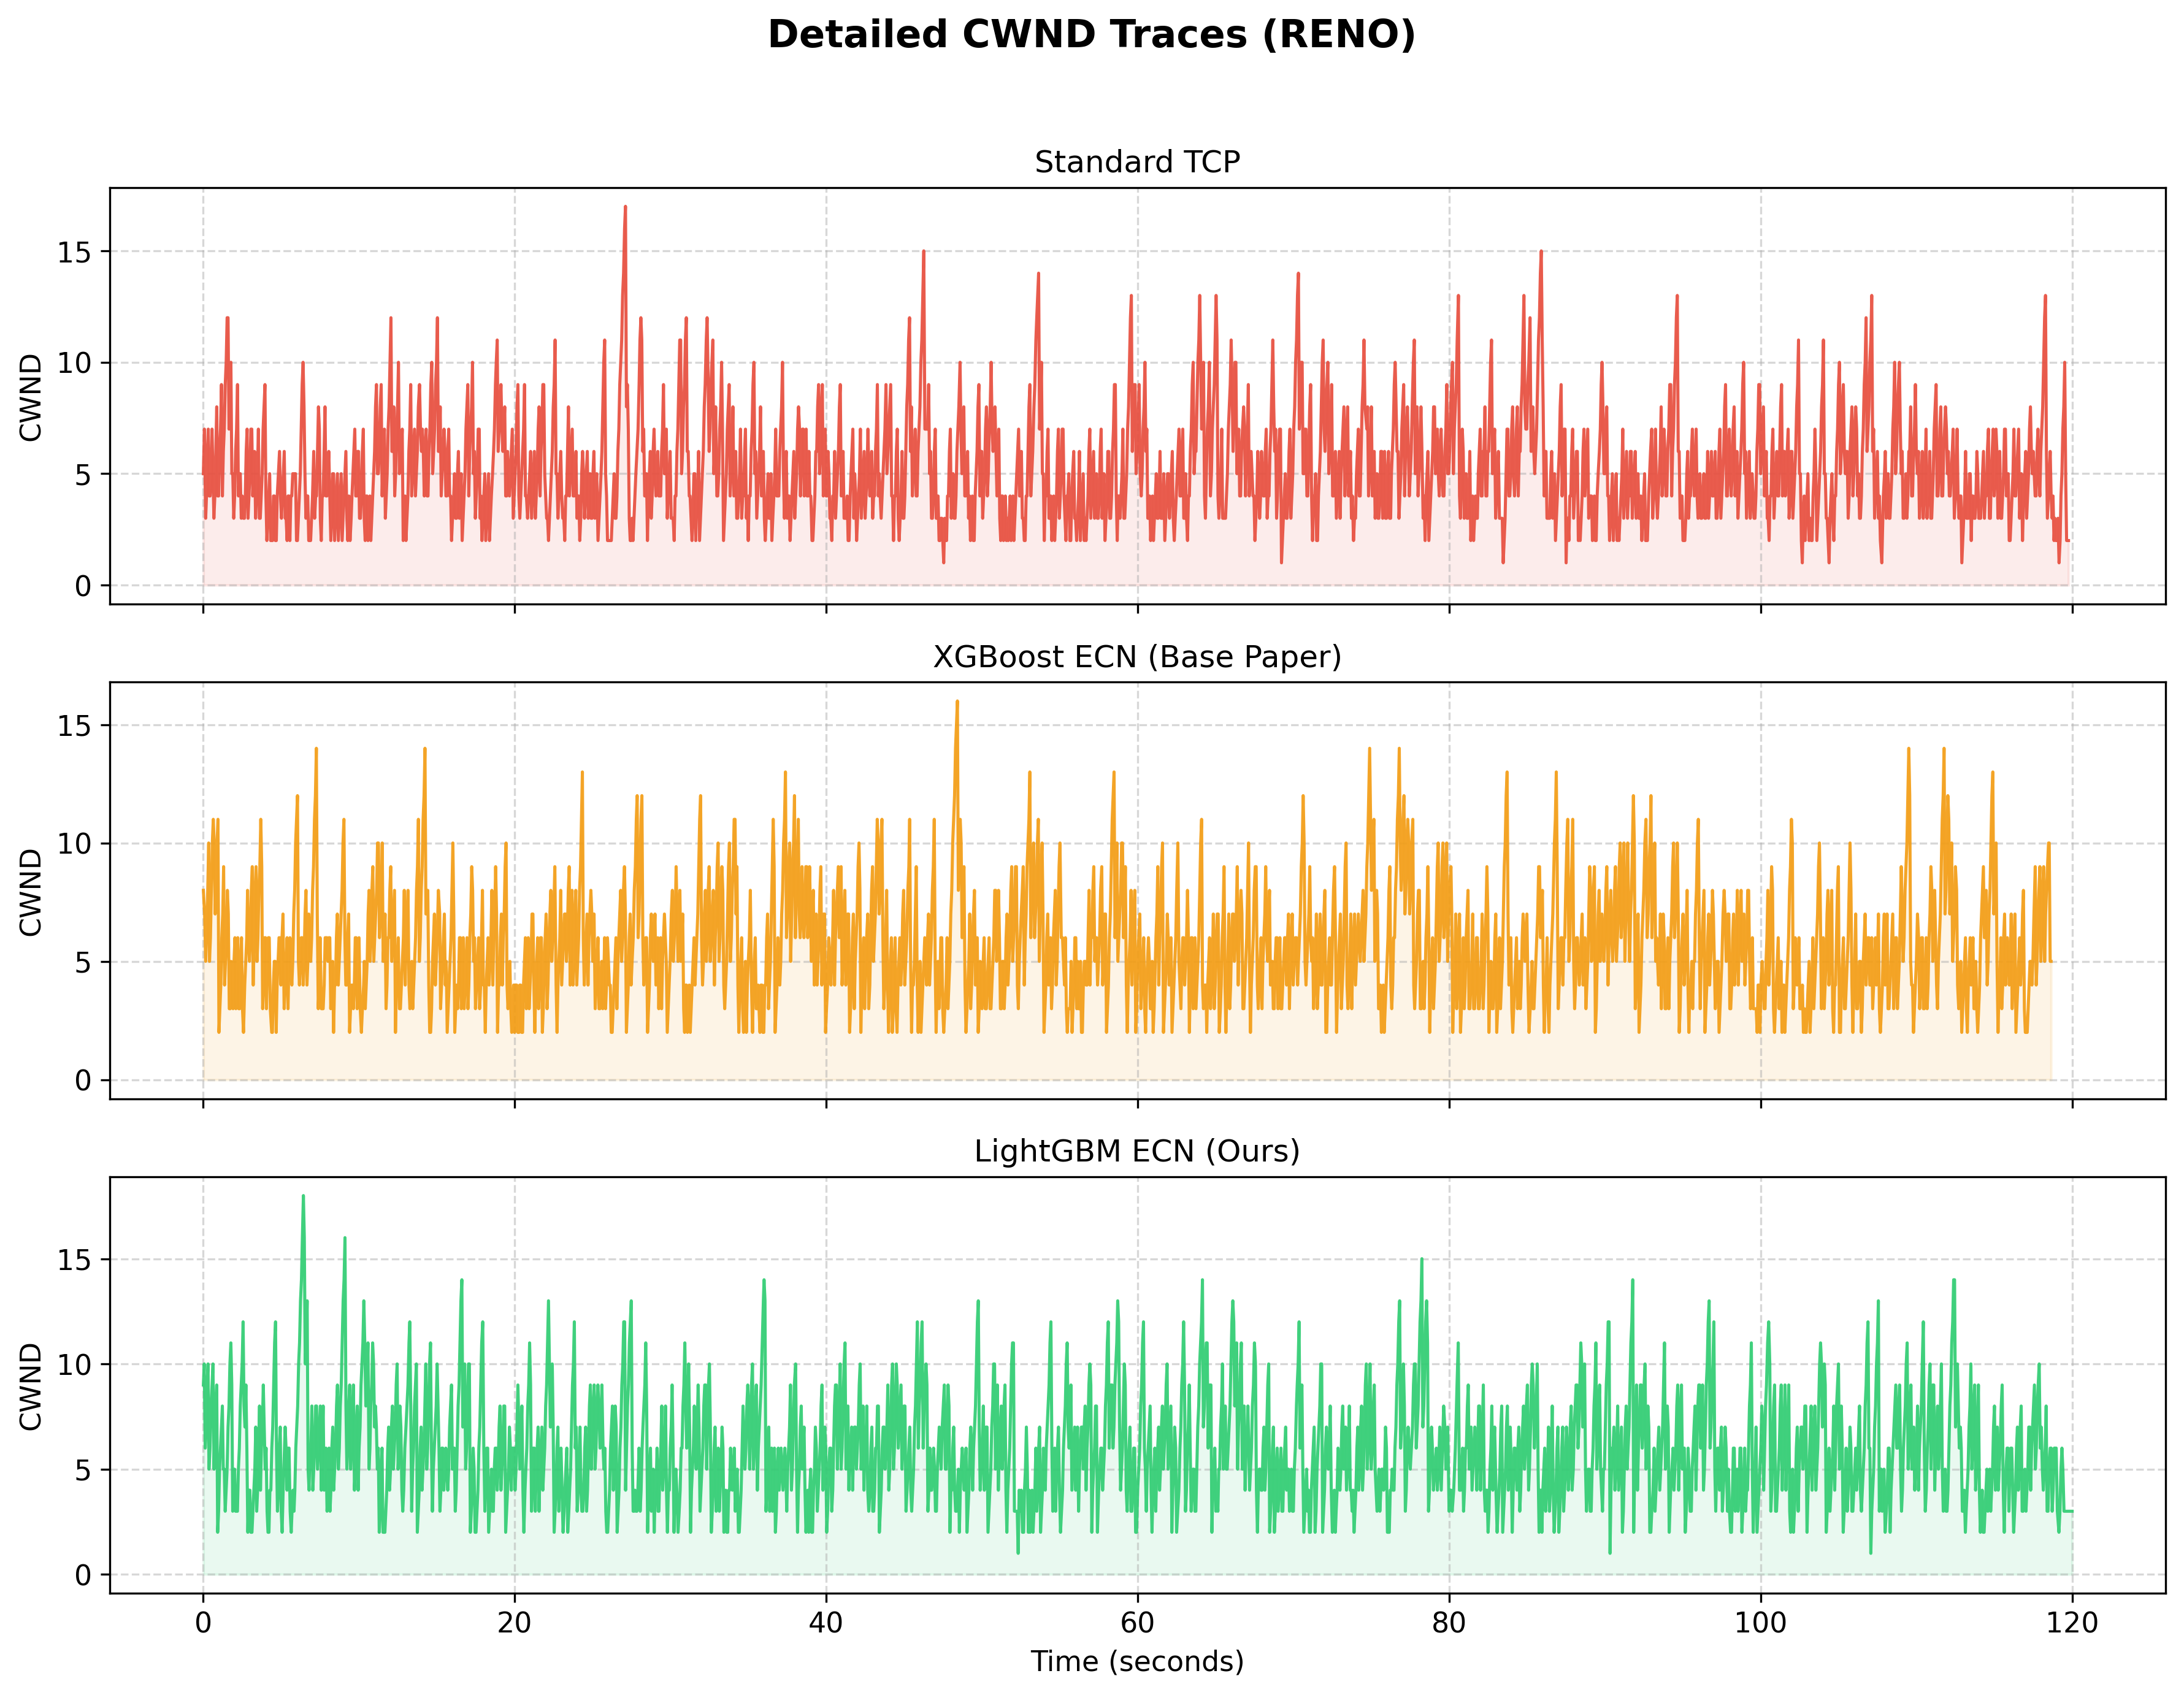
\includegraphics[width=\columnwidth]{cwnd_trace(Reno).png}
\caption{Congestion window (CWND) trace for TCP Reno across Baseline, Binary ECN, and Proportional ECN conditions over the 120\,s experiment duration.}
\label{fig:cwnd_reno}
\end{figure}

% Fig. 5 — CWND trace for TCP Cubic
\begin{figure}[H]
\centering
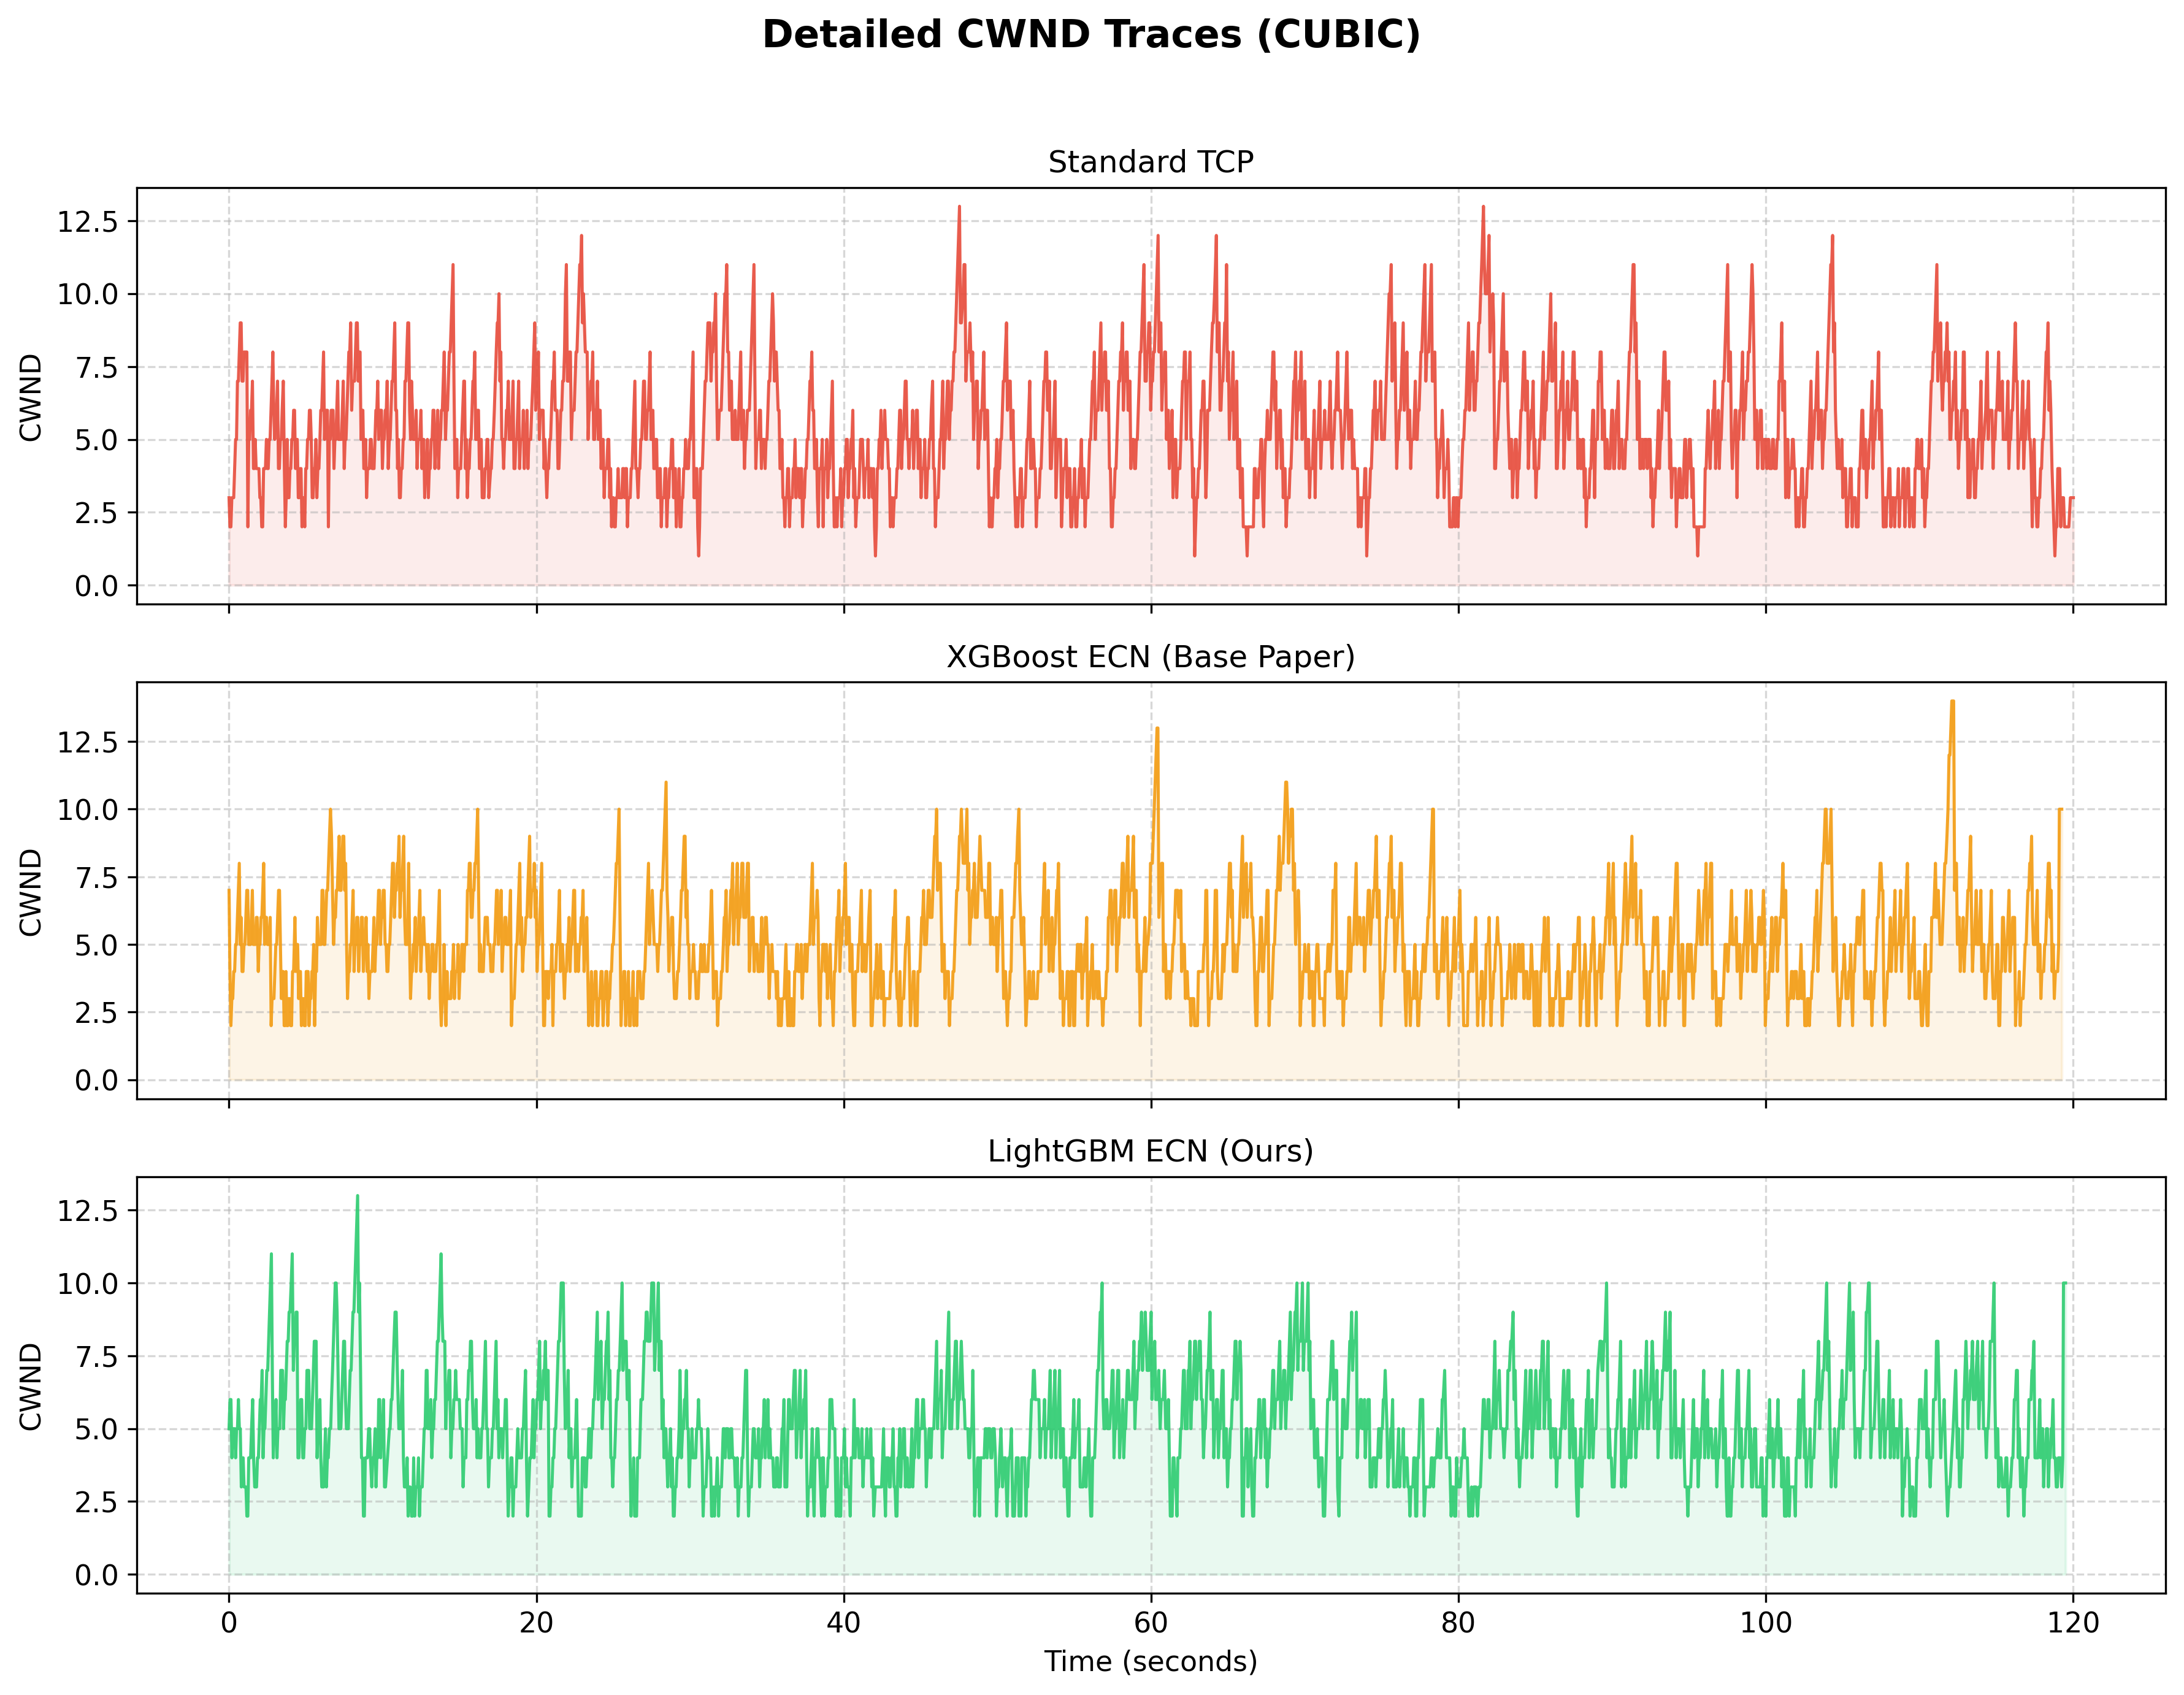
\includegraphics[width=\columnwidth]{cwnd_trace(cubic).png}
\caption{Congestion window (CWND) trace for TCP Cubic across Baseline, Binary ECN, and Proportional ECN conditions over the 120\,s experiment duration.}
\label{fig:cwnd_cubic}
\end{figure}

\subsection{Comparative Summary}

% --- TABLE VIII ---
\begin{table}[ht]
\renewcommand{\arraystretch}{1.3}
\caption{Overall System Performance}
\label{tab:summary}
\centering
\footnotesize
\begin{tabularx}{\columnwidth}{@{}L L@{}}
\toprule
\textbf{Dimension} & \textbf{Our System} \\
\midrule
Dataset size       & 57,808 rows (combined Reno+Cubic) \\
Models trained     & Single unified Reno+Cubic model \\
Label strategy     & Multi-signal consensus (leak-free) \\
Class balance      & 48.07\% positive / 51.93\% negative \\
Features           & 71 engineered / 45 retained \\
Best model F1      & 0.9723 (LightGBM) \\
ECN mechanism      & \texttt{tc qdisc} proportional RED adjustment \\
Deployment threshold & 0.56 (calibrated) \\
Reno throughput gain & $+15.5\%$ vs.\ baseline \\
Cubic retransmissions & 0 (100\% elimination) + best CWND stability \\
ECN signals (Reno) & 18 proactive signals \\
\bottomrule
\end{tabularx}
\end{table}

Three core findings emerge from the results. First, the labeling strategy is the single most impactful design decision: the multi-signal consensus approach produces a well-separated, naturally balanced class boundary that enables high-fidelity classification (F1\,=\,0.9723) without relying on aggressive oversampling. Second, proportional ECN at the queue-management level delivers superior performance compared to binary packet-marking: for Reno it activates proactively (18 signals) and delivers higher throughput; for Cubic it achieves additional CWND smoothing beyond passive AQM. Third, training a single unified model across both CC variants generalizes successfully---confirmed by the near-identical $\sim$28,900 Reno and Cubic sample counts contributing equally to the F1\,=\,0.9723 result, eliminating the need for per-algorithm model specialization.

% -------------------------------------------------------------------
\section{Conclusion}
\label{sec:conclusion}
% -------------------------------------------------------------------

This paper presented a proactive TCP congestion control system that combines real-time ML-based loss prediction with proportional RED queue management to prevent packet loss before it occurs. Three key contributions distinguish the work: a multi-signal consensus labeling strategy that eliminates data leakage and produces a naturally balanced training set; a single LightGBM model trained on combined Reno and Cubic data with 71 engineered features (45 retained after automated selection); and a proportional artificial ECN mechanism that adjusts RED thresholds continuously as a function of prediction confidence.

The effectiveness of the approach has been shown by experimental results on Mininet. In the case of TCP Cubic, the system has removed all the retransmissions ($755 \rightarrow 0$) and has increased CWND stability by 11.3\% relative to the uncontrolled baseline. In the case of TCP Reno, the throughput enhancement is 15.5\% due to maintaining a greater average congestion window with proactive congestion signaling. The proportional LightGBM mechanism in both instances outperforms the binary ECN approach, showing the usefulness of confidence-proportional queue management.

It is also determined in the work that the single unified model, trained on both Reno and Cubic variants, has been shown to generalize successfully, without requiring specialization of the model per-algorithm. This is one step towards a more generally applicable predictive congestion system that can be expanded to other CC algorithms without re-training.

Several limitations remain. Every experiment is run in a controlled Mininet that uses a fixed bottleneck of 10\,Mbit/s with a 30\,ms RTT; real-world networks are even more variable in terms of the background traffic patterns, RTT dynamics, and path asymmetry. The system should be tested on the higher-bandwidth paths, cellular and WiFi link types, and different competing flow counts in the future. Generalizability claims would be further reinforced with training on real Internet traces, e.g., MAWI or CAIDA datasets. Furthermore, further enhancements of throughput-stability trade-offs might be achieved by extending the proportional control mechanism to be used to adjust per-flow pacing rate, not only to RED thresholds.


% -------------------------------------------------------------------
\begin{thebibliography}{17}


\bibitem{rfc5681}
E.~Blanton, V.~Paxson, and M.~Allman, \textit{TCP Congestion Control}, RFC 5681, Sep. 2009.

\bibitem{rfc9438}
L.~Xu, S.~Ha, I.~Rhee, V.~Goel, and L.~Eggert, \textit{CUBIC for Fast and Long-Distance Networks}, RFC 9438, Aug. 2023.

\bibitem{rfc3168}
S.~Floyd, K.~Ramakrishnan, and D.~Black, \textit{The Addition of Explicit Congestion Notification (ECN) to IP}, RFC 3168, Sep. 2001.

\bibitem{manet}
O.~J.~Adaramola and J.~R.~Olasina, ``Machine Learning-Driven Congestion Prediction in Mobile Ad-Hoc Networks Through Modelling Approaches,'' 2023.

\bibitem{ptcl}
A.~Akhtar, I.~Zafar, M.~A.~Zaki, and M.~Khurram, ``Machine Learning-based fixed access Network Interface Congestion Prediction,'' \textit{Pakistan Journal of Engineering, Technology \& Science}, vol.~12, no.~1, pp.~26--36, 2024.

\bibitem{stgcn}
B.~Magar, R.~Kulkarni, V.~Khatavkar, and H.~Vanjari, ``Predictive network congestion management for enterprise systems: a graph neural network approach with operational insights,'' 2025.

\bibitem{ali2024}
I.~Ali, S.~Hong, and T.~Cheung, ``Congestion or no congestion: Packet loss identification and prediction using machine learning,'' in \textit{Proc. 16th Int. Conf. on Platform Technology and Service (PlatCon)}, 2024, pp.~1--6.

\bibitem{labonne}
M.~Labonne, C.~Chatzinakis, and A.~Olivereau, ``Predicting Bandwidth Utilization on Network Links Using Machine Learning,'' in \textit{Proc. 2020 European Conference on Networks and Communications (EuCNC)}, 2020, pp.~242--247.

\bibitem{wide2025}
Y.~Wang, ``Advanced Network Traffic Prediction Using Deep Learning Techniques: A Comparative Study of SVR, LSTM, GRU, and Bidirectional LSTM Models,'' \textit{ITM Web of Conferences}, vol.~70, 2025.

\bibitem{rl_mesh}
S.~Mahajan, P.~Srideviponmalar, R.~Harikrishnan, and K.~Kotecha, ``Reinforcement Learning Based Congestion Control Technique for Wireless Mesh Networks,'' \textit{International Journal of Networked and Distributed Computing}, 2025.

\bibitem{dqn_tcp}
E.~A\v{g}lamazlar, E.~Eken, and H.~B.~Ge\c{c}ici, ``A Deep Reinforcement Learning-Based TCP Congestion Control Algorithm: Design, Simulation, and Evaluation,'' \textit{arXiv preprint}, 2026.

\bibitem{aqm_lstm}
C.~A.~Gomez, X.~Wang, and A.~Shami, ``Intelligent Active Queue Management Using Explicit Congestion Notification,'' in \textit{Proc. 2019 IEEE Global Communications Conference (GLOBECOM)}, 2019.

\bibitem{remora}
A.~Kumar and N.~Hemrajani, ``Optimized Extreme Gradient Boosting with Remora Algorithm for Congestion Prediction in Transport Layer,'' \textit{International Journal of Computer Network and Information Security}, vol.~16, no.~3, 2024.

\bibitem{ccn}
P.~Bazmi and M.~Keshtgary, ``A Neural Network Based Congestion Control Algorithm for Content-Centric Networks,'' \textit{Journal of Advanced Computer Science \& Technology}, 2014.

\bibitem{wsn}
G.-W.~Lee, S.-Y.~Lee, and E.-N.~Huh, ``Congestion Prediction Modeling for Quality of Service Improvement in Wireless Sensor Networks,'' \textit{Sensors}, vol.~14, no.~5, 2014.

\bibitem{tafa_survey}
Z.~Tafa and V.~Milutinovic, ``Machine Learning in Congestion Control: A Survey on Selected Algorithms and a New Roadmap to their Implementation,'' \textit{arXiv preprint arXiv:2112.15522}, 2021.

\bibitem{welzl2024}
M.~Welzl, S.~Islam, and M.~von Stephanides, ``Real-Time TCP Packet Loss Prediction Using Machine Learning,'' \textit{IEEE Access}, vol.~12, pp.~159622--159634, 2024. DOI: 10.1109/ACCESS.2024.3488511.

\end{thebibliography}

\end{document}